% !TeX root = RJwrapper.tex
\title{Ari: The Automated R Instructor}
\author{by Sean Kross, Jeffrey T. Leek, John Muschelli}

\maketitle

\abstract{%
We present the \texttt{ari} package for automatically generating
technology-focused educational videos. The goal of the package is to
create reproducible videos, with the ability to change and update video
content seamlessly. We present several examples of generating videos
including using R Markdown slide decks, PowerPoint slides, or simple
images as source material. We also discuss how \texttt{ari} can help
instructors reach new audiences through programmatically translating
materials into other languages.
}

% Any extra LaTeX you need in the preamble

\hypertarget{introduction}{%
\subsection{Introduction}\label{introduction}}

Videos are a crucial way people learn and they are pervasive in online
education platforms (Hsin and Cigas 2013; Hartsell and Yuen 2006).
Producing educational videos with a lecturer speaking over slides takes
time, energy, and usually video editing skills. Maintaining the accuracy
and relevancy of lecture videos focused on technical subjects like
computing programming or data science can often require remaking an
entire video, requiring extensive editing and splicing of new segments.
We present \CRANpkg{ari}, the \textbf{A}utomated \textbf{R}
\textbf{I}nstructor as a tool to address these issues by creating
reproducible presentations and videos that can be automatically
generated from plain text files or similar artifacts. By using
\pkg{ari}, we provide a tool for users to rapidly create and update
video content.

In its simplest form a lecture video is comprised of visual content
(e.g.~slides and figures) and a spoken explanation of the visual
content. Instead of a human lecturer, the \pkg{ari} package uses a
text-to-speech system to synthesize spoken audio for a lecture. Modern
text-to-speech systems that take advantage of recent advancements in
artificial intelligence research are available from
\href{https://cloud.google.com/text-to-speech/}{Google},
\href{https://azure.microsoft.com/en-us/services/cognitive-services/text-to-speech/}{Microsoft},
and \href{https://aws.amazon.com/polly/}{Amazon}. Many of these
synthesizers make use of deep learning methods, such as WaveNet (Van Den
Oord et al. 2016) and have interfaces in R (Edmondson 2019; Muschelli
2019a; Leeper 2017). Currently in \pkg{ari}, synthesis of the the audio
can be rendered using any of these services through the
\CRANpkg{text2speech} package (Muschelli 2019b). The default is
\href{https://aws.amazon.com/polly/}{Amazon Polly}, which has
text-to-speech voice generation in over twenty one languages,
implemented in the \CRANpkg{aws.polly} package (Leeper 2017). In
addition to multiple languages, the speech generation services provide
voices with several pitches representing different genders within the
same language. We present the \pkg{ari} package with reproducible use
case examples and the video outputs with different voices in multiple
languages.

The \pkg{ari} package relies on the \CRANpkg{tuneR} package for
splitting and combining audio files appropriately so that lecture
narration is synced with each slide (Ligges et al. 2018). Once the audio
is generated, it is synced with images to make a lecture video. Multiple
open source tools for video editing and splicing exist; \pkg{ari} takes
advantage of the \texttt{ffmpeg} (\url{http://www.ffmpeg.org/})
software, a command-line interface to the \texttt{libav} library. These
powerful tools have been thoroughly tested with a development history
spanning almost 20 years. \pkg{ari} has been built with presets for
\texttt{ffmpeg} which allow output videos to be compatible with multiple
platforms, including the YouTube and Coursera players. These presets
include specifying the bitrate, audio and video codecs, and the output
video format. The numerous additional video specifications for
customization can be applied to command-line arguments \texttt{ffmpeg}
through \pkg{ari}.

We have developed a workflow with \pkg{ari} as the centerpiece for
automatically generating educational videos. The narration script for
lecture videos is stored in a plain text format, so that it can be
synthesized into audio files via text-to-speech services. By storing
lecture narration in plain text it can be updated, tracked, and
collaboratively or automatically updated with version control software
like Git and GitHub. If the figures in the lecture slides are created in
a reproducible framework, such as generated using R code, the entire
video can be reproducibly created and automatically updated. Thus,
\pkg{ari} is the Automated R Instructor. We will provide examples of
creating videos based on the following sets of source files: a slide
deck built with R Markdown, a set of images and a script, or a Google
Slide deck or PowerPoint presentation.\\
The overview of the processes demonstrated in this paper are seen in
Figure \ref{fig:fig1}. We will also demonstrate the \CRANpkg{ariExtra},
which contains helper functions extensions of \pkg{ari}.

\begin{Schunk}
\begin{figure}
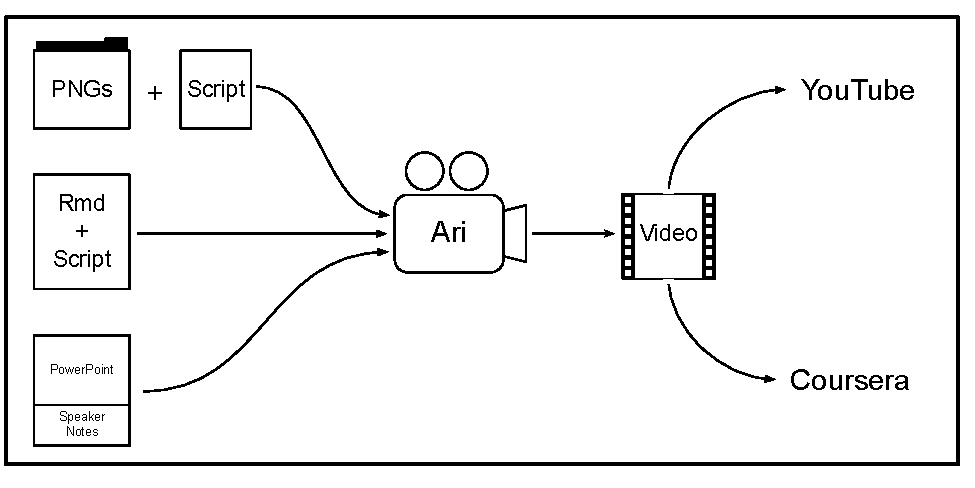
\includegraphics[width=1\linewidth]{Figure-1-Ari-pdf} \caption[Ari is designed to fit into several existing workflows for creating lectures and presentations]{Ari is designed to fit into several existing workflows for creating lectures and presentations. Videos can be created with Ari from a series of images and a narrative script, from an R Markdown document, or from a PowerPoint presentation with speaker notes. Ari is pre-configured so that videos are ready to be uploaded to popular platforms like YouTube or Coursera.}\label{fig:fig1}
\end{figure}
\end{Schunk}

\hypertarget{configuring-ari}{%
\subsection{Configuring Ari}\label{configuring-ari}}

Ari relies on several software packages including FFmpeg, one of the
most popular libraries for processing audio, video, and image files.
Configuring FFmpeg can be challenging, therefore we have provided a
Docker image so that Ari users can start producing videos quickly. A
guide to getting started with Docker and using our Docker image is
included with Ari as a vignette which can be accessed via
\texttt{vignette("Simple-Ari-Configuration-with-Docker")}. Users who are
interested in configuring Ari on their own may find the Dockerfile
associated with the guide useful, and it is being actively developed at
\url{https://github.com/seankross/ari-on-docker}.

\hypertarget{making-videos-with-ari-ari_stitch}{%
\subsection{\texorpdfstring{Making videos with \texttt{ari}:
\texttt{ari\_stitch}}{Making videos with ari: ari\_stitch}}\label{making-videos-with-ari-ari_stitch}}

The main workhorse of \pkg{ari} is the \texttt{ari\_stitch} function.
This function requires an ordered set of images and an ordered set of
audio objects, either paths to \texttt{wav} files or \pkg{tuneR} Wave
objects, that correspond to each image. The \texttt{ari\_stitch}
function sequentially ``stitches'' each image in the video for the
duration of its corresponding audio object using \texttt{ffmpeg}. In
order to use \pkg{ari}, one must have an \texttt{ffmpeg} installation to
combine the audio and images. Other packages such as \CRANpkg{animation}
have a similar requirement. Moreover, on
\href{https://www.shinyapps.io/}{shinyapps.io}, a dependency on the
\pkg{animation} package will trigger an installation of \texttt{ffmpeg}
so \pkg{ari} can be used on
\href{https://www.shinyapps.io/}{shinyapps.io}. In the example below, 2
images (packaged with \pkg{ari}) are overlaid withe white noise for
demonstration. This example also allows users to check if the output of
\texttt{ffmpeg} works with a desired video player.

\begin{Schunk}
\begin{Sinput}
library(tuneR)
library(ari)
result = ari_stitch(
  ari_example(c("mab1.png", "mab2.png")),
  list(noise(), noise()),
  output = "noise.mp4")
isTRUE(result)
\end{Sinput}
\end{Schunk}

\begin{Schunk}
\begin{Soutput}
[1] TRUE
\end{Soutput}
\end{Schunk}

The output is a logical indicator, but additional attributes are
available, such as the path of the output file:

\begin{Schunk}
\begin{Sinput}
attributes(result)$outfile
\end{Sinput}
\end{Schunk}

\begin{Schunk}
\begin{Soutput}
[1] "noise.mp4"
\end{Soutput}
\end{Schunk}

The video for this output can be seen at
\url{https://youtu.be/3kgaYf-EV90}.

\hypertarget{synthesizer-authentication}{%
\subsection{Synthesizer
authentication}\label{synthesizer-authentication}}

The above example uses \texttt{tuneR::noise()} to generate audio and to
show that any audio object can be used with \pkg{ari}. In most cases
however, \pkg{ari} is most useful when combined with synthesizing audio
using a text-to-speech system. Though one can generate the spoken audio
in many ways, such as fitting a custom deep learning model, we will
focus on using the aforementioned services (e.g.~Amazon Polly) as they
have straightforward public web APIs. One obstacle in using such
services is that users must go through steps to provide authentication,
whereas most of these APIs and the associated R packages do not allow
for interactive authentication such as OAuth.

The \pkg{text2speech} package provides a unified interface to these 3
text-to-speech services, and we will focus on Amazon Polly and its
authentication requirements. Polly is authenticated using the
\CRANpkg{aws.signature} package (Leeper 2019). The \pkg{aws.signature}
documentation provides options and steps to create the relevant
credentials; we have also provided an additional
\href{http://seankross.com/2017/05/02/Access-Amazon-Web-Services-in-R.html}{tutorial}.
Essentially, the user must sign up for the service and retrieve public
and private API keys and put them into their R profile or other areas
accessible to R. Running
\texttt{text2speech::tts\_auth(service\ =\ "amazon")} will indicate if
authentication was successful (if using a different service, change the
\texttt{service} argument). NB: The APIs are generally paid services,
but many have free tiers or limits, such as Amazon Polly's free tier for
the first year (\url{https://aws.amazon.com/polly/pricing/}).

\hypertarget{creating-speech-from-text-ari_spin}{%
\subsection{\texorpdfstring{Creating Speech from Text:
\texttt{ari\_spin}}{Creating Speech from Text: ari\_spin}}\label{creating-speech-from-text-ari_spin}}

After Polly has been authenticated, videos can be created using the
\texttt{ari\_spin} function with an ordered set of images and a
corresponding ordered set of text strings. This text is the ``script''
that is spoken over the images to create the output video. The number of
elements in the text needs to be equal to the number of images. Let us
take a part of Mercutio's speech from Shakespeare's Romeo and Juliet
(Shakespeare 2003) and overlay it on two images from the Wikipedia page
about Mercutio (\url{https://en.wikipedia.org/wiki/Mercutio}):

\begin{Schunk}
\begin{Sinput}
speech =  c(
  "I will now perform part of Mercutio's speech from Shakespeare's Romeo and Juliet.", 
  "O, then, I see Queen Mab hath been with you.
   She is the fairies' midwife, and she comes
   In shape no bigger than an agate-stone
   On the fore-finger of an alderman,
   Drawn with a team of little atomies
   Athwart men's noses as they lies asleep;")
mercutio_file = "death_of_mercutio.png"
mercutio_file2 = "mercutio_actor.png"
\end{Sinput}
\end{Schunk}

\begin{Schunk}
\begin{Sinput}
shakespeare_result = ari_spin(
  c(mercutio_file, mercutio_file2),
  speech, output = "romeo.mp4", voice = "Joanna")
isTRUE(shakespeare_result)
\end{Sinput}
\end{Schunk}

\begin{Schunk}
\begin{Soutput}
[1] TRUE
\end{Soutput}
\end{Schunk}

The speech output can be seen at \url{https://youtu.be/SFhvM9gI0kE}.\\
We chose the voice ``Joanna'' which is designated as a female sounding
US-English speaker for the script. Each voice is language-dependent; we
can see the available voices for English for Amazon Polly at
\url{https://docs.aws.amazon.com/polly/latest/dg/SupportedLanguage.html}.

Though the voice generation is relatively clear, we chose a
Shakespearean example to demonstrate the influence and production value
of the variety of dialects available from these text-to-speech services.
Compare the video of ``Joanna'' to the same video featuring ``Brian''
who ``speaks'' with a British English dialect:

\begin{Schunk}
\begin{Sinput}
gb_result = ari_spin(
  c(mercutio_file, mercutio_file2),
  speech, output = "romeo_gb.mp4", voice = "Brian")
isTRUE(gb_result)
\end{Sinput}
\end{Schunk}

\begin{Schunk}
\begin{Soutput}
[1] TRUE
\end{Soutput}
\end{Schunk}

The resulting video can be seen at \url{https://youtu.be/fSS0JSb4VxM}.

The output video format is MP4 by default, but several formats can be
specified via specifying the appropriate ``muxer'' for \texttt{ffmpeg}
(see the function \texttt{ffmpeg\_muxers}). Supported codecs can be
founded using the functions \texttt{ffmpeg\_audio\_codecs} and
\texttt{ffmpeg\_video\_codecs}. Additional options can be passed to
\texttt{ffmpeg} from \texttt{ari\_stitch} and \texttt{ari\_spin} to
customize the video to the necessary specifications.

We now discuss the number of image and script inputs that \pkg{ari} is
designed to work with, including text files and a series of PNG images,
a Google Slide deck or a PowerPoint presentation with the script written
in the speaker notes section, or an HTML slide presentation created from
an R Markdown, where the script is written in the HTML comments.

\hypertarget{creating-videos-from-r-markdown-documents}{%
\subsubsection{Creating Videos from R Markdown
Documents}\label{creating-videos-from-r-markdown-documents}}

Many R users have experience creating slide decks with R Markdown, for
example using the \CRANpkg{rmarkdown} or \CRANpkg{xaringan} packages
(Allaire et al. 2019; Xie, Allaire, and Grolemund 2018; Xie 2018). In
\pkg{ari}, the HTML slides are rendered using \CRANpkg{webshot} (Chang
2018) and the script is located in HTML comments (i.e.~between
\texttt{\textless{}!-\/-} and \texttt{-\/-\textgreater{}}). For example,
in the file \texttt{ari\_comments.Rmd} included in \pkg{ari}, which is
an \texttt{ioslides} type of R Markdown slide deck, we have the last
slide:

\begin{Schunk}
\begin{Sinput}
x = readLines(ari_example("ari_comments.Rmd"))
tail(x[ x != ""], 4)
\end{Sinput}
\begin{Soutput}
[1] "## Conclusion"                                             
[2] "<!--"                                                      
[3] "Thank you for watching this video and good luck using Ari!"
[4] "-->"                                                       
\end{Soutput}
\end{Schunk}

so that the first words spoken on that slide are \texttt{"Thank\ you"}.
This setup allows for one plain text, version-controllable, integrated
document that can reproducibly generate a video. We believe these
features allow creators to make agile videos, that can easily be updated
with new material or changed when errors or typos are found. Moreover,
this framework provides an opportunity to translate videos into multiple
languages, we will discuss in the future directions.

Using \texttt{ari\_narrate}, users can create videos from R Markdown
documents that create slide decks. The can be passed in, and the output
will be created using the \texttt{render} function from \pkg{rmarkdown}
(Allaire et al. 2019). If the slides are already rendered, the user can
pass these slides and the original document, where the script is
extracted. Passing rendered slides allows with the option for a custom
rendering script. Here we create the video for
\texttt{ari\_comments.Rmd}, where the slides are rendered inside
\texttt{ari\_narrate}:

\begin{Schunk}
\begin{Sinput}
# Create a video from an R Markdown file with comments and slides
res = ari_narrate(
  script = ari_example("ari_comments.Rmd"),
  voice = "Kendra",
  capture_method = "iterative")
\end{Sinput}
\end{Schunk}

The output video is located at \url{https://youtu.be/rv9fg_qsqc0}. In
our experience with several users we have found that some HTML slides
take more or less time to render when using \pkg{webshot}; for example
they may be tinted with gray because they are in the middle of a slide
transition when the image of the slide is captured. Therefore we provide
the \texttt{delay} argument in \texttt{ari\_narrate} which is passed to
\pkg{webshot}. This can resolve these issues by allowing more time for
the page to fully render, however this means it may take for more time
to create each video. We also provide the argument
\texttt{capture\_method} to allow for finely-tuned control of
\texttt{webshot}. When \texttt{capture\_method\ =\ "vectorized"},
\pkg{webshot} is run on the entire slide deck in a faster process,
however we have experienced slide rendering issues with this setting
depending on the configuration of an individual's computer. However when
\texttt{capture\_method\ =\ "iterative"}, each slide is rendered
individually in \texttt{webshot}, which solves many rendering issues,
however it causes videos to be rendered more slowly.\\
In the future, other HTML headless rendering engines (\texttt{webshot}
uses PhantomJS) may be used if they achieve better performance, but we
have found \pkg{webshot} to work well in most of our applications.

With respect to accessibility, \pkg{ari} encourages video creators to
type out a script by design. This provides an effortless source of
subtitles for people with hearing loss rather than relying on other
services, such as YouTube, to provide speech-to-text subtitles. When
using \texttt{ari\_spin}, if the \texttt{subtitles} argument is
\texttt{TRUE}, then an SRT file for subtitles will be created with the
video.

One issue with synthesis of technical information is that changes to the
script are required for Amazon Polly or other services to provide a
correct pronunciation. For example, if you want the service to say
``RStudio'' or ``ggplot2'', the phrases ``R Studio'' or ``g g plot 2''
must be written exactly that way in the script. These phrases will then
appear in an SRT subtitle file, which may be confusing to a viewer.
Thus, some post-processing of the SRT file may be needed.

\hypertarget{creating-videos-from-other-documents}{%
\subsubsection{Creating Videos from Other
Documents}\label{creating-videos-from-other-documents}}

In order to create a video from a Google Slide deck or PowerPoint
presentation, the slides should be converted to a set of images. We
recommend using the PNG format for these images. In order to get the
script for the video, we suggest putting the script for each slide in
the speaker notes section of that slide. Several of the following
features for video generation are in our package \pkg{ariExtra}
(\url{https://github.com/muschellij2/ariExtra}). The speaker notes of
slides can be extracted using \CRANpkg{rgoogleslides} (Noorazman 2018)
for Google Slides via the API or using
\CRANpkg{readOffice}/\CRANpkg{officer} (Gohel 2019; Ewing 2017) to read
from PowerPoint documents. Google Slides can be downloaded as a PDF and
converted to PNGs using the \CRANpkg{pdftools} package (Ooms 2019). The
\pkg{ariExtra} package also has a \texttt{pptx\_notes} function for
reading PowerPoint notes. Converting PowerPoint files to PDF can be done
using LibreOffice and the \CRANpkg{docxtractr} package (Rudis and Muir
2019) which contains the necessary wrapper functions.

To demonstrate this, we use an example PowerPoint is located on Figshare
(\url{https://figshare.com/articles/Example_PowerPoint_for_ari/8865230}).
We can convert the PowerPoint to PDF, then to a set of PNG images, then
extract the speaker notes.

\begin{Schunk}
\begin{Sinput}
pptx = "ari.pptx"
download.file(paste0("https://s3-eu-west-1.amazonaws.com/", 
                     "pfigshare-u-files/16252631/ari.pptx"),
              destfile = pptx)
pdf = docxtractr::convert_to_pdf(pptx) # >= 0.6.2 
pngs = pdftools::pdf_convert(pdf, dpi = 300)
notes = ariExtra::pptx_notes(pptx)
notes
\end{Sinput}
\end{Schunk}

\begin{Schunk}
\begin{Soutput}
[1] "Sometimes it’s hard for an instructor to take the time to record their lectures.
For example, I’m in a coffee shop and it may be loud."

[2] "Here is an example of a plot with really small axes.  We plot the x versus the y
-variables and a smoother between them."
\end{Soutput}
\end{Schunk}

The \pkg{ariExtra} package also can combine these processes and take
multiple input types (Google Slides, PDFs, PPTX) and harmonize the
output. The \texttt{pptx\_to\_ari} function combines the above steps:

\begin{Schunk}
\begin{Sinput}
doc = ariExtra::pptx_to_ari(pptx)
\end{Sinput}
\end{Schunk}

\begin{verbatim}
Converting page 1 to /var/folders/1s/wrtqcpxn685_zk570bnx9_rr0000gr/T/
/Rtmpo6aD9u/filede6236136195.png... done!
Converting page 2 to /var/folders/1s/wrtqcpxn685_zk570bnx9_rr0000gr/T/
/Rtmpo6aD9u/filede62326b98ef.png... done!
\end{verbatim}

\begin{Schunk}
\begin{Sinput}
doc[c("images", "script")]
\end{Sinput}
\end{Schunk}

\begin{verbatim}
$images
[1] "/private/var/folders/1s/wrtqcpxn685_zk570bnx9_rr0000gr/T/
Rtmpo6aD9u/filede6236058cc5_files/slide_1.png"
[2] "/private/var/folders/1s/wrtqcpxn685_zk570bnx9_rr0000gr/T/
Rtmpo6aD9u/filede6236058cc5_files/slide_2.png"
$script
[1] "Sometimes it’s hard for an instructor to take the time to record their lectures. 
For example, I’m in a coffee shop and it may be loud."
[2] "Here is an example of a plot with really small axes. We plot the x versus the 
y-variables and a smoother between them."
\end{verbatim}

which can be passed to \texttt{ari\_spin}.

We can then render the video with the ``Kimberly'' voice. We use the
\texttt{divisible\_height} argument to forcibly scale the height of the
images to be divisible by 2 if necessary. This is required by the
\texttt{x264} (default) codec which we have specified as a preset:

\begin{Schunk}
\begin{Sinput}
pptx_result = ari_spin(pngs, notes, output = "pptx.mp4", voice = "Kimberly",
    divisible_height = TRUE, subtitles = TRUE)
isTRUE(pptx_result)
\end{Sinput}
\end{Schunk}

You can see the output at \url{https://youtu.be/TBb3Am6xsQw}. Here we
can see the first few lines of the subtitle file:

\begin{Schunk}
\begin{Soutput}
[1] "1"                                       
[2] "00:00:00,000 --> 00:00:02,025"           
[3] "Sometimes it’s hard for an instructor to"
[4] "2"                                       
[5] "00:00:02,025 --> 00:00:04,005"           
[6] "take the time to record their lectures." 
\end{Soutput}
\end{Schunk}

For Google Slides, the slide deck can be downloaded as a PowerPoint and
the previous steps can be used, however it can also be downloaded
directly as a PDF. We will use the same presentation, but uploaded to
Google Slides. The \pkg{ariExtra} package has the function
\texttt{gs\_to\_ari} to wrap this functionality (as long as link sharing
is turned on), where we can pass the Google identifier:

\begin{Schunk}
\begin{Sinput}
gs_doc = ariExtra::gs_to_ari("14gd2DiOCVKRNpFfLrryrGG7D3S8pu9aZ")
\end{Sinput}
\begin{Soutput}
Converting page 1 to /tmp/Rtmpu3DQSM/file1d634b862a77.png... done!
Converting page 2 to /tmp/Rtmpu3DQSM/file1d636aba2d36.png... done!
\end{Soutput}
\end{Schunk}

Note, as Google provides a PDF version of the slides, this obviates the
LibreOffice dependency.

Alternatively, the notes can be extracted using \pkg{rgoogleslides} and
for Google Slides via the API, but requires authentication, so we will
omit it here. Thus, we should be able to create videos using R Markdown,
Google Slides, or PowerPoint presentations in an automatic fashion.

\hypertarget{summary}{%
\subsection{Summary}\label{summary}}

The \pkg{ari} package combines multiple open-source tools and APIs to
create reproducible workflows for creating videos. These videos can be
created using R Markdown documents, PowerPoint presentations, Google
Slide decks, or simply series of images. The audio overlaid on the
images can be separate or contained within the storage of the images.
These workflows can then be reproduced in the future and easily updated.
As the current voice synthesis options are somewhat limited in the
tenacity and inflection given, we believe that educational and
informational videos are the most applicable area.

\hypertarget{future-directions}{%
\subsection{Future directions}\label{future-directions}}

The \pkg{ari} package is already being used to build data science
curricula (Kross and Guo 2019) and we look forward to collaborating with
video creators to augment \pkg{ari} according to their changing needs.
In the following section we outline possible directions for the future
of the project.

Since \pkg{ari} is designed for teaching technical content, we plan to
provide better support for the pronunciation of technical terms like the
names of popular software tools. These names are usually not pronounced
correctly by text-to-speech services because they are not words
contained in the training data used in the deep learning models used by
these services. To address this concern we plan to compile a dictionary
of commonly used technical terms and the phonetic phrasing and spelling
of these terms that are required in order to achieve the correct
pronunciation from text-to-speech services.

In addition to still images and synthesized voices, we would like to
develop new technologies for incorporating other automatically generated
videos into lectures generated by \pkg{ari}. As computer programming,
statistics, and data science instructors we often rely on live coding
(Chen and Guo 2019) to demonstrate software tools to our students. Live
coding videos suffer from many of the same problems as other kinds of
technical videos as we addressed in the introduction. Therefore we plan
to build a system for automating the creation of live coding videos.
These videos would also be created using plain text documents like R
Markdown. They would integrate synthesized narration with code chunks
that would be displayed and executed according to specialized commands
that would specify when code should be executed in an IDE like RStudio.
These commands could also control which panes and tabs of the IDE are
visible or emphasized.

As programmatic video creation software improves, we plan to extend
\pkg{ari} so it can expand its compatibility with different
technologies. For example we believe the heavy reliance on an
\texttt{ffmpeg} installation can be mitigated in the future with
advances in the \pkg{av} package. Though the \pkg{av} package has
powerful functionality and is currently porting more from \texttt{libav}
and therefore \texttt{ffmpeg}, it currently does not have the
capabilities required for \pkg{ari}. Although third party installation
from \url{https://ffmpeg.org/} can be burdensome to a user, package
managers such as \texttt{brew} for OSX and \texttt{choco} for Windows
provide an easier installation and configuration experience.

Although we rely on Amazon Polly for voice synthesis, other packages
provide voice synthesis, such as \CRANpkg{mscstts} for Microsoft and
\CRANpkg{googleLanguageR} for Google. We created the \pkg{text2speech}
package to harmonize these synthesis options for \pkg{ari}. Thus,
switching from one voice generation service to another simply involves
switching the \texttt{service} and \texttt{voice} arguments in
\pkg{ari}, assuming the service is properly authenticated. This ease of
switching allows researchers to compare and test which voices and
services are most effective at delivering content.

We see significant potential in how \pkg{ari} could expand global
learning opportunities. Video narration scripts can be automatically
translated into other languages with services like the
\href{https://cloud.google.com/translate/docs/}{Google Translation API},
where \pkg{googleLanguageR} provides an interface. Amazon Polly can
speak languages other than English, meaning that one can write a lecture
once and generate lecture videos in multiple languages. Therefore this
workflow can greatly expand the potential audience for educational
videos with relatively little additional effort from lecture creators.
We plan to flesh out these workflows so that video creators can manage
videos in multiple languages. We hope to add functionality so that
communities of learners with language expertise can easily suggest
modifications to automatically translated videos, and tooling so
suggestions can be incorporated quickly.

\hypertarget{bibliography}{%
\subsection{Bibliography}\label{bibliography}}

\bibliography{RJreferences}

\hypertarget{refs}{}
\leavevmode\hypertarget{ref-rmarkdown}{}%
Allaire, JJ, Yihui Xie, Jonathan McPherson, Javier Luraschi, Kevin
Ushey, Aron Atkins, Hadley Wickham, Joe Cheng, Winston Chang, and
Richard Iannone. 2019. \emph{rmarkdown: Dynamic Documents for R}.
\url{https://rmarkdown.rstudio.com}.

\leavevmode\hypertarget{ref-webshot}{}%
Chang, Winston. 2018. \emph{webshot: Take Screenshots of Web Pages}.
\url{https://CRAN.R-project.org/package=webshot}.

\leavevmode\hypertarget{ref-ChenLAS2019}{}%
Chen, Charles, and Philip J. Guo. 2019. ``Improv: Teaching Programming
at Scale via Live Coding.'' In \emph{Proceedings of the Sixth Annual Acm
Conference on Learning at Scale}. L@S '19. New York, NY, USA: ACM.
\url{https://doi.org/10.1145/3330430.3333627}.

\leavevmode\hypertarget{ref-googleLanguageR}{}%
Edmondson, Mark. 2019. \emph{googleLanguageR: Call Google's 'Natural
Language' API, 'Cloud Translation' API, 'Cloud Speech' API and 'Cloud
Text-to-Speech' API}.

\leavevmode\hypertarget{ref-readOffice}{}%
Ewing, Mark. 2017. \emph{readOffice: Read Text Out of Modern Office
Files}. \url{https://CRAN.R-project.org/package=readOffice}.

\leavevmode\hypertarget{ref-officer}{}%
Gohel, David. 2019. \emph{officer: Manipulation of Microsoft Word and
PowerPoint Documents}. \url{https://CRAN.R-project.org/package=officer}.

\leavevmode\hypertarget{ref-hartsell2006video}{}%
Hartsell, Taralynn, and Steve Chi-Yin Yuen. 2006. ``Video Streaming in
Online Learning.'' \emph{AACE Journal} 14 (1). Association for the
Advancement of Computing in Education (AACE): 31--43.

\leavevmode\hypertarget{ref-hsin2013short}{}%
Hsin, Wen-Jung, and John Cigas. 2013. ``Short Videos Improve Student
Learning in Online Education.'' \emph{Journal of Computing Sciences in
Colleges} 28 (5). Consortium for Computing Sciences in Colleges:
253--59.

\leavevmode\hypertarget{ref-Kross-2019}{}%
Kross, Sean, and Philip J. Guo. 2019. ``End-User Programmers Repurposing
End-User Programming Tools to Foster Diversity in Adult End-User
Programming Education.'' In \emph{Proceedings of VL/HCC 2019: IEEE
Symposium on Visual Languages and Human-Centric Computing}. VL/HCC '19.
Memphis, TN, USA.

\leavevmode\hypertarget{ref-aws.polly}{}%
Leeper, Thomas J. 2017. \emph{aws.polly: Client for AWS Polly}.

\leavevmode\hypertarget{ref-aws.signature}{}%
---------. 2019. \emph{aws.signature: Amazon Web Services Request
Signatures}.

\leavevmode\hypertarget{ref-tuneR}{}%
Ligges, Uwe, Sebastian Krey, Olaf Mersmann, and Sarah Schnackenberg.
2018. \emph{tuneR: Analysis of Music and Speech}.
\url{https://CRAN.R-project.org/package=tuneR}.

\leavevmode\hypertarget{ref-mscstts}{}%
Muschelli, John. 2019a. \emph{mscstts: R Client for the Microsoft
Cognitive Services 'Text-to-Speech' REST API}.
\url{https://CRAN.R-project.org/package=mscstts}.

\leavevmode\hypertarget{ref-text2speech}{}%
---------. 2019b. \emph{text2speech: Text to Speech}.
\url{https://github.com/muschellij2/text2speech}.

\leavevmode\hypertarget{ref-rgoogleslides}{}%
Noorazman, Hairizuan Bin. 2018. \emph{rgoogleslides: R Interface to
Google Slides}. \url{https://CRAN.R-project.org/package=rgoogleslides}.

\leavevmode\hypertarget{ref-pdftools}{}%
Ooms, Jeroen. 2019. \emph{pdftools: Text Extraction, Rendering and
Converting of PDF Documents}.
\url{https://CRAN.R-project.org/package=pdftools}.

\leavevmode\hypertarget{ref-docxtractr}{}%
Rudis, Bob, and Chris Muir. 2019. \emph{docxtractr: Extract Data Tables
and Comments from Microsoft Word Documents}.
\url{http://gitlab.com/hrbrmstr/docxtractr}.

\leavevmode\hypertarget{ref-shakespeare2003romeo}{}%
Shakespeare, William. 2003. \emph{Romeo and Juliet}. Cambridge
University Press.

\leavevmode\hypertarget{ref-van2016wavenet}{}%
Van Den Oord, Aäron, Sander Dieleman, Heiga Zen, Karen Simonyan, Oriol
Vinyals, Alex Graves, Nal Kalchbrenner, Andrew W Senior, and Koray
Kavukcuoglu. 2016. ``WaveNet: A Generative Model for Raw Audio.''
\emph{SSW} 125.

\leavevmode\hypertarget{ref-xaringan}{}%
Xie, Yihui. 2018. \emph{xaringan: Presentation Ninja}.
\url{https://CRAN.R-project.org/package=xaringan}.

\leavevmode\hypertarget{ref-rmarkdownbook}{}%
Xie, Yihui, J.J. Allaire, and Garrett Grolemund. 2018. \emph{R Markdown:
The Definitive Guide}. Boca Raton, Florida: Chapman; Hall/CRC.
\url{https://bookdown.org/yihui/rmarkdown}.

\bibliography{RJreferences.bib}

\address{%
Sean Kross\\
Department of Cognitive Science, University of California, San Diego\\
9500 Gilman Dr.\\ La Jolla, CA 92093\\
}
\href{mailto:seankross@ucsd.edu}{\nolinkurl{seankross@ucsd.edu}}

\address{%
Jeffrey T. Leek\\
Department of Biostatistics, Johns Hopkins Bloomberg School of Public
Health\\
615 N Wolfe Street\\ Baltimore, MD 21231\\
}
\href{mailto:jtleek@jhu.edu}{\nolinkurl{jtleek@jhu.edu}}

\address{%
John Muschelli\\
Department of Biostatistics, Johns Hopkins Bloomberg School of Public
Health\\
615 N Wolfe Street\\ Baltimore, MD 21231\\
}
\href{mailto:jmusche1@jhu.edu}{\nolinkurl{jmusche1@jhu.edu}}

